\begin{figure}[h!]
     \centering
     \begin{subfigure}[h]{0.7\textwidth}
         \centering
         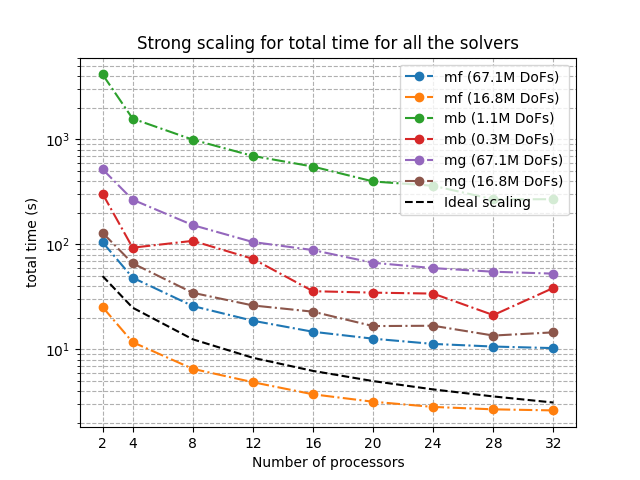
\includegraphics[width=\textwidth]{figure/strongcomp_total.png}
         \caption{Total time}
     \end{subfigure}
     \begin{subfigure}[h]{0.5\textwidth}
         \centering
         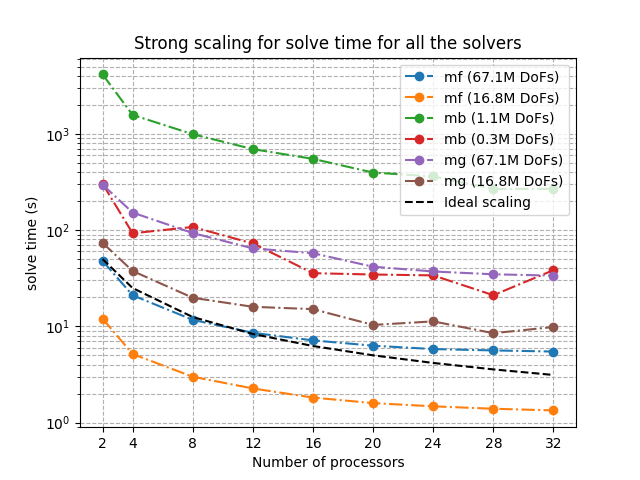
\includegraphics[width=\textwidth]{figure/strongcomp_solve.png}
         \caption{Solve time}
     \end{subfigure}
     \hspace*{-0.4cm}
     \begin{subfigure}[h]{0.5\textwidth}
         \centering
         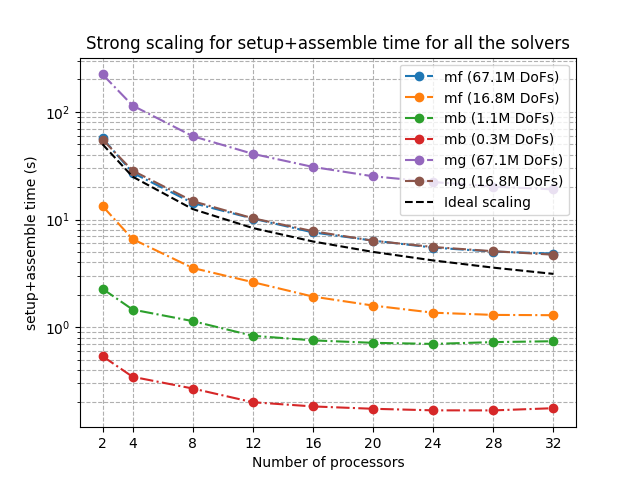
\includegraphics[width=\textwidth]{figure/strongcomp_setup+assemble.png}
         \caption{Setup and assemble time}
     \end{subfigure}
     \caption{Total, solve, and setup+assemble time scaling comparison between all the solvers for the two highest problem sizes. Strong scaling can be compared with the reference lines, weak scaling can be assessed knowing that each plot differs quadruplicates the problem size.}
     \label{fig:strongcomp}
\end{figure}
